\section{Data}
\label{sec:data}
\subsection{Data Source}
\label{sec:data_source}
The data we used for this project came from the Sloan Digital Sky Survey (SDSS) Data Release (DR)7~\cite{abazajian2009seventh}, and the Galaxy Zoo (GZ) project first data release~\cite{lintott2010galaxy}. 
SDSS is a major multi-spectral imaging and spectroscopic redshift survey using a dedicated wide-field 2.5 m telescope located at Apache Point Observatory (APO) near Sacramento Peak in Southern New Mexico.
DR7 contains five-band photometry for 357 million distinct objects~\cite{abazajian2009seventh}. 
The GZ project collected simple morphological classifications of nearly 900,000 galaxies drawn from SDSS DR7, contributed by hundreds of thousands of volunteers~\cite{lintott2010galaxy}. 

We took the galaxy names and classifications from the GZ database, and searched SDSS for the corresponding images. For each galaxy five FITS files are provided by SDSS.
The SDSS images are unique in that the data is stored in five bands (`ugriz') instead of the typical three channels (RGB). 
`ugriz' channels are also absolute, rather than relative, meaning that instead of ranging from 0 to 255, the pixels have any integer greater than zero. 
This is so that the actual intensity of the galaxy in a specific band can be extracted in order to calculate galaxy mass and composition.


\begin{figure}[h!]
	\centering
	\captionsetup{justification=centering}
	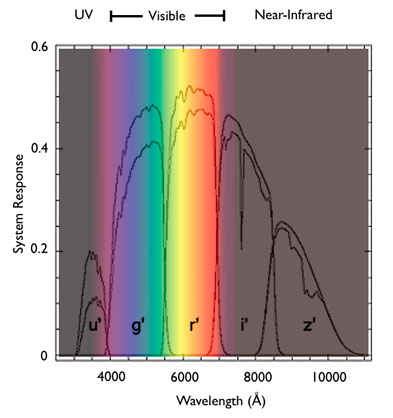
\includegraphics[scale=0.5]{Figures/filters.jpg}
	\caption{The `ugriz' filter schematic with a colour spectrum plotted on top.}
	\label{fig:filters}
\end{figure}



\subsection{Pre-processing}
Since the classifications in GZ are from crowdsourcing, we only used the data entries that
have high confidence classifications. We choose galaxies with debiased probability (given in~\cite{lintott2010galaxy}) greater than 0.985 for spiral galaxies, and 0.926 for elliptical galaxies, respectively. 
We choose these thresholds to ensure that: (i) the galaxies used for training the neural network have highly accurate classifications; and (ii) the number of data for both classes in the training and test sets are balanced~\cite{khan2019deep}. We obtained 19306 and 18811 galaxies for spiral and elliptical respectively. 

The data we got from SDSS are in Flexible Image Transport System (FITS) format. 
Each FITS file contains a header part and a data part. We removed the header part and resized the images to $200 \times 200$ pixels. As we discussed in Section~\ref{sec:data_source}, `ugriz' covers a broader band than RGB images. Common ways to map `ugriz' files to RGB images would take 3 or 4 channels (out of 5) of `ugriz', and do a linear transformation on them, thus would definitely lose some information. 
In order to keep a more complete data for each galaxy we used `ugriz' files rather than RGB images as the input to our classifier. Figure~\ref{fig:ugriz} shows the gray-scale images of the u, g, r, i and z band photometry of a spiral galaxy as well as the RGB image of the same galaxy. We can see that there is information on each band but the RGB image only uses 3 or 4 of them which would cause information loss.

\begin{figure}[h]
	\centering
	\captionsetup{justification=centering}
	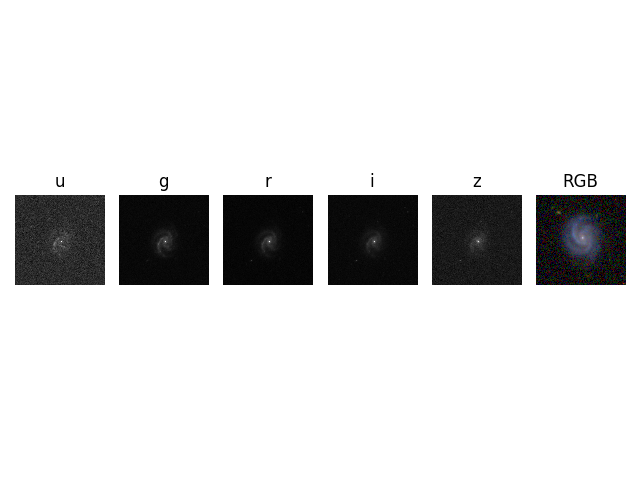
\includegraphics[trim={0 4cm 0 4cm},clip]{Figures/ugriz_vs_rgb.png}
	\caption{The 'ugriz' images and the RGB image of the same galaxy}
	\label{fig:ugriz}
\end{figure}

